% !TeX program = xelatex
\documentclass[aspectratio=169]{beamer}

\usepackage{babel}
\usepackage{graphicx}
\usepackage{subcaption}
\usepackage{hyperref}
\usepackage{amsmath}
\usepackage{algorithm}
\usepackage{algpseudocode}
\usepackage{fontspec}
\usepackage{listings}
\usepackage{xcolor}
\usepackage{adjustbox}
\usepackage{capt-of}

\usefonttheme{professionalfonts}

\algrenewcommand\textproc{\textsf}

\setbeamertemplate{caption}[numbered]
\setbeamersize{text margin left=6mm, text margin right=6mm}

\lstdefinestyle{code}{
  language=Python,
  basicstyle=\ttfamily\footnotesize,
  numbers=left, numberstyle=\tiny, stepnumber=1,
  frame=single,
  breaklines=true,
  tabsize=2,
  showstringspaces=false,
  keywordstyle=\color{blue},
  commentstyle=\color{gray},
  stringstyle=\color{orange}
}
\lstset{style=code}

\graphicspath{{images/}}

\title{PCDVQ report}
\author{Li Daniil}
\institute{Skoltech}
\date{2025}

\begin{document}

    \frame{\titlepage}
    \section{PCDVQ}

\begin{frame}{Polar Coordinate Decoupling Vector Quantization (PCDVQ)}
    \begin{columns}
        \column{0.55\textwidth}
            \centering
            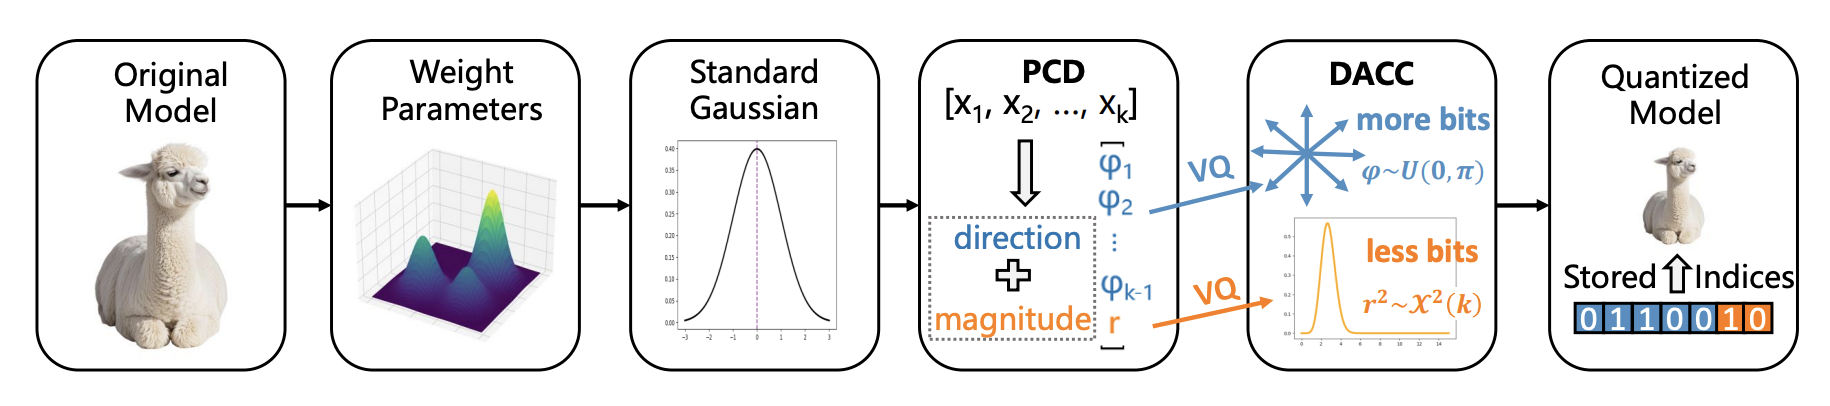
\includegraphics[width=\linewidth,height=0.34\textheight,keepaspectratio]{pipeline.png}
            \captionof{figure}{The pipeline of PCDVQ}\label{fig:pipeline}
            \vspace{0.5em}

            \begin{minipage}{\linewidth}
                \centering
                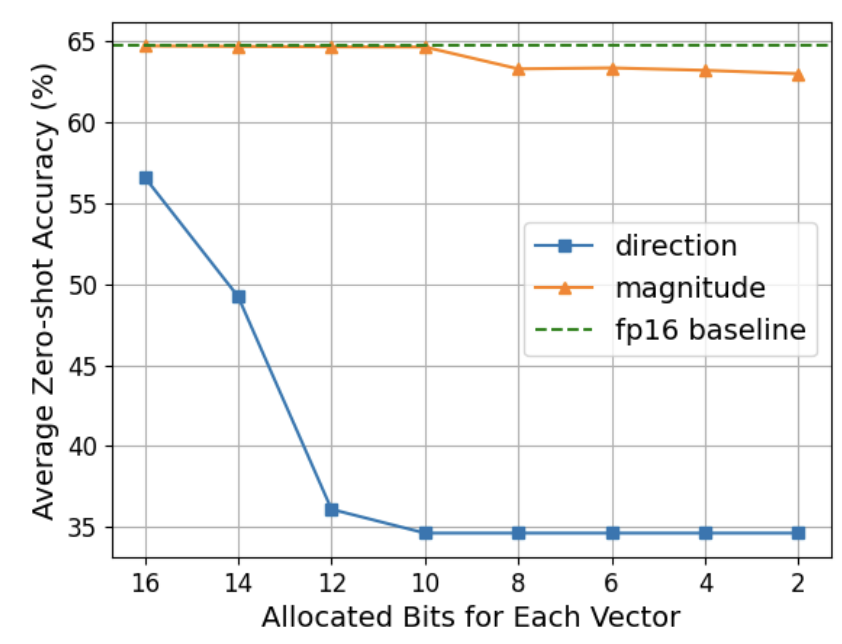
\includegraphics[width=0.49\linewidth,height=0.4\textheight,keepaspectratio]{sensitivity_gap.png}\hfill
                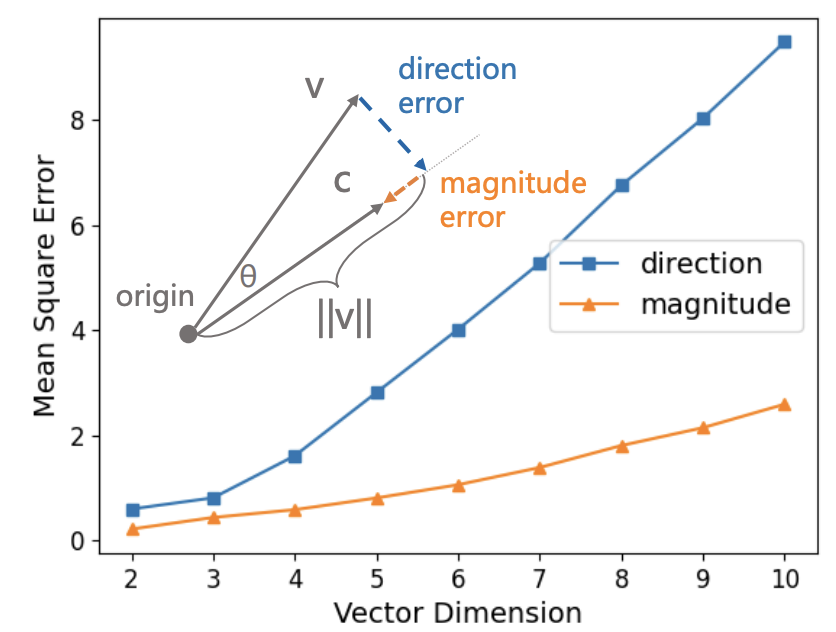
\includegraphics[width=0.49\linewidth,height=0.4\textheight,keepaspectratio]{error_diff.png}\\
                {\captionof{figure}{Compare direction and magnitude}\label{fig:compare_dir_magn}}
            \end{minipage}

        \column{0.45\textwidth}
            This method consist of the next stages (Fig.~\ref{fig:pipeline}):
            \begin{itemize}
                \item Standard Gaussian Regularization (SGR). They used Random Hadamard Transformation (RHT) for SGR
                \item Polar Coordinate Decoupling (PCD)
                \item Distribution Aligned Codebook Construction (DACC)
            \end{itemize}

            Motivation: direction is identified to be more essential than magnitude (Fig.~\ref{fig:compare_dir_magn})
    \end{columns}
\end{frame}

    \section{Implementation}

\begin{frame}{Implementation}
    \small

    Implementation: \url{https://github.com/danlee65071/pcdvq/tree/main}

    \vspace{0.4em}
    \begin{itemize}\setlength{\itemsep}{2pt}\setlength{\parskip}{0pt}
        \item Model: Qwen3-4B
        \item Dataset: WikiText2
    \end{itemize}

    The approach was tested with $a=5$, $b=2$ (bits for direction/magnitude).
    Authors used $a\in\{14,16\}$ and $b=2$ (Fig.~\ref{fig:bit_setting}).

    $k=64$ was used for the first reshape (original weights) and $k=8$ for directions.
    In the paper $k$ for weights was $8$ (Fig.~\ref{fig:bit_setting}).

    \vspace{0.4em}
    \centering
    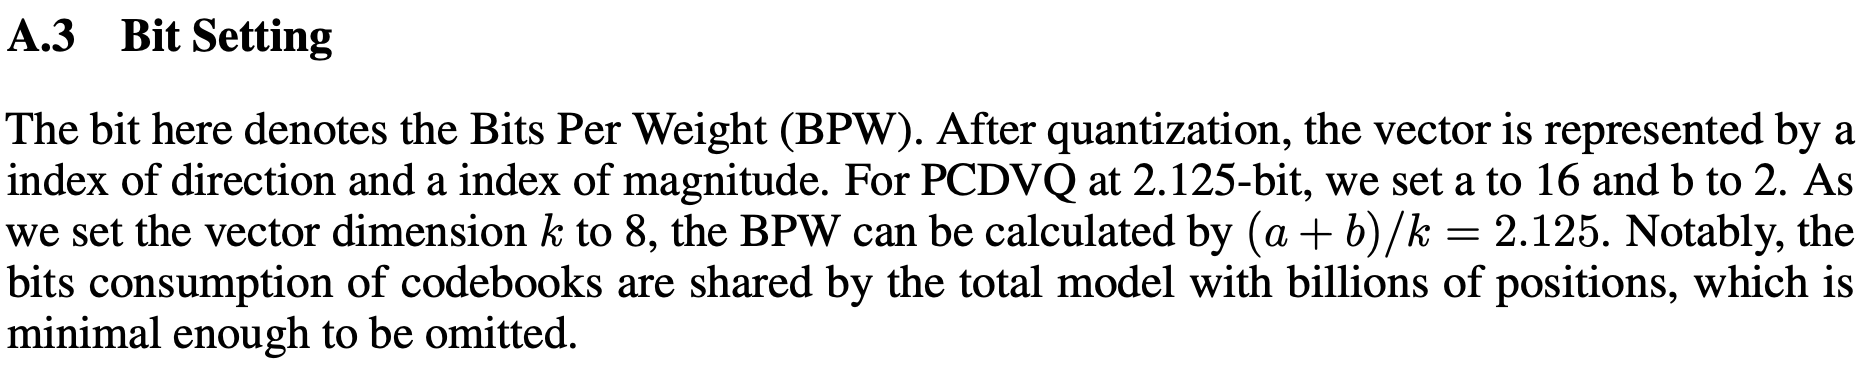
\includegraphics[width=0.9\linewidth,height=0.42\textheight,keepaspectratio]{bit_setting.png}

    \captionof{figure}{From the paper: bit settings}\label{fig:bit_setting}
\end{frame}

    \section{FWHT}

\begin{frame}{Implementation of the fast Walsh Hadamard transform (FWHT)}
    \begin{columns}
        \column{0.55\textwidth}
            \begin{algorithm}[H]
                \caption{Fast Walsh–Hadamard Transform}
                \begin{algorithmic}[1]
                    \Procedure{fwht}{$a$}
                    \State $n \gets |a|$, \textbf{assert} $n$ — power of $2$
                    \State $h \gets 1$
                    \While{$h < n$}
                        \For{$i \gets 0;\ i < n;\ i \gets i + 2h$}
                        \For{$j \gets i;\ j < i+h;\ j \gets j+1$}
                            \State $x \gets a[j]$; $y \gets a[j+h]$
                            \State $a[j] \gets x+y$; \quad $a[j+h] \gets x-y$
                        \EndFor
                        \EndFor
                        \State  divide $a[\cdot]$ by $\sqrt{2}$; \quad $h \gets 2h$
                    \EndWhile
                    \EndProcedure
                \end{algorithmic}\label{alg:fwht}
            \end{algorithm}
        
        \column{0.45\textwidth}
            \small
            A random Hadamard transformation is used to bring the weights to SGR.\@
            \textbf{Fast Walsh–Hadamard transform (FWHT)} is an efficient algorithm to compute the Walsh–Hadamard transform (WHT). This algorithm has a complexity of $O(n\log n)$ (Algorithm~\ref{alg:fwht}).\\
            The \textbf{hadamard-transform} python package was used (\url{https://github.com/amitport/hadamard-transform}).\\
            Forward and reverse applications are identical

    \end{columns}

\end{frame}

    \section{PCD}


\begin{frame}[fragile]{Implementation of the polar coordinates decoupling (PCD). To polar}
  \begin{columns}[T,onlytextwidth]
    \column{0.55\textwidth}
      \begin{adjustbox}{max height=0.65\textheight,keepaspectratio}
\begin{lstlisting}[language=Python, basicstyle=\ttfamily\scriptsize, aboveskip=2pt, belowskip=2pt, numbers=left, numberstyle=\tiny, frame=single, breaklines=true]
def to_polar(x: torch.Tensor) -> Tuple[torch.Tensor, torch.Tensor]:
    p, k = x.shape
    magnitudes = torch.linalg.vector_norm(x, dim=1, keepdim=True)
    phis = torch.empty(p, k-1, dtype=x.dtype, device=x.device)
    x_squares = x * x
    x_squares_flipped = torch.flip(x_squares, dims=[1])
    x_squares_cumsum_flipped = torch.cumsum(x_squares_flipped, dim=1)
    x_squares_cumsum = torch.flip(x_squares_cumsum_flipped, dims=[1])
    y_head = x_squares_cumsum[:, 1:-1].sqrt()
    x_head = x[:, :-2]
    phis[:, :-1] = torch.atan2(y_head, x_head)
    phi_last = torch.atan2(x[:, -1], x[:, -2])
    phi_last = (phi_last + 2 * math.pi) % (2 * math.pi)
    phis[:, -1] = phi_last
    return phis, magnitudes.squeeze(-1)
\end{lstlisting}
      \end{adjustbox}
    \column{0.4\textwidth}
        The following transformation to spherical coordinates was implemented\\
        This function converts the vector representation $x$ from Cartesian coordinates to polar coordinates: it calculates the norm (modulus) of each vector and the angles between the axes using arctangents. For the last two coordinates, the angle is additionally adjusted so that it always lies in the range $(0,2\pi]$
  \end{columns}
\end{frame}

    \section{PCD_to_polar}


\begin{frame}[fragile]{Implementation of the polar coordinates decoupling (PCD). To cartesian}
    \begin{columns}[T,onlytextwidth]
        \column{0.55\textwidth}
        \begin{adjustbox}{max height=0.65\textheight,keepaspectratio}
\begin{lstlisting}[language=Python, basicstyle=\ttfamily\scriptsize, aboveskip=2pt, belowskip=2pt, numbers=left, numberstyle=\tiny, frame=single, breaklines=true]
def get_unit_directions(directions: torch.Tensor) -> torch.Tensor:
    sin_matrix = torch.sin(directions)
    cos_matrix = torch.cos(directions)
    cum_sin = torch.cumprod(sin_matrix, dim=-1)
    sin_prefix = torch.cat([torch.ones_like(sin_matrix[:, :1]), cum_sin[:, :-1]], dim=-1)
    x_except_last = sin_prefix * cos_matrix
    x_last = cum_sin[:, -1:].clone()
    unitary_directions = torch.cat([x_except_last, x_last], dim=-1)
    return unitary_directions

def to_cartesian(phis: torch.Tensor, r: torch.Tensor) -> torch.Tensor:
    if r.ndim == 1:
        r = r.unsqueeze(-1)
    unit_dirs = PCDVQ.get_unit_directions(phis)
    x = r * unit_dirs
    return x
\end{lstlisting}
        \end{adjustbox}
    \column{0.4\textwidth}
        $get\_unit\_directions$: constructs a unit direction vector based on sets of angles in hyperspherical coordinates. Takes $\cos$ for each axis, accumulates the products of $\sin $ from left to right, and obtains the components as $sin\_prefix\cdot\cos $, and the last one as the full product of $\sin $\\
        $to\_cartesian$: сonverts the radius $r$ to a column if necessary, calculates unit directions via $get\_unit\_directions(phis)$, and multiplies them by $r$\\
  \end{columns}
\end{frame}

    \section{E8_lattice}


\begin{frame}[fragile]{\texorpdfstring{$E_8$}{E8} lattice}
  \begin{columns}[T,onlytextwidth]
    \column{0.55\textwidth}
      \begin{adjustbox}{max height=0.55\textheight,keepaspectratio}
\begin{lstlisting}[language=Python, basicstyle=\ttfamily\scriptsize, aboveskip=2pt, belowskip=2pt, numbers=left, numberstyle=\tiny, frame=single, breaklines=true]
def e8_minimal_directions(device=None, dtype=torch.float16, normalize=False):
    eye_matrix = torch.eye(8, dtype=dtype, device=device)
    row_idxs, col_idxs = torch.triu_indices(8, 8, offset=1, dtype=torch.int64, device=device)
    e1, e2 = eye_matrix[row_idxs], eye_matrix[col_idxs]
    int_roots = torch.cat([e1 + e2, e1 - e2, -e1 + e2, -e1 - e2], 0)
    signs = torch.tensor([-1.0, 1.0], dtype=dtype, device=device)
    halfs = torch.cartesian_prod(*([signs] * 8)).reshape(-1, 8)
    half_roots = 0.5 * halfs[(halfs.prod(dim=-1) > 0)]
    e8_roots = torch.cat([int_roots, half_roots], dim=0)
    if normalize:
        e8_roots = e8_roots / math.sqrt(2.0)
    return e8_roots
\end{lstlisting}
      \end{adjustbox}

    \column{0.4\textwidth}
      The \texorpdfstring{$E_8$}{E8} lattice can be described as all points in \(\mathbb{R}^8\) such that either all coordinates are integers or all are half-integers, and the sum of coordinates is even:
      \scriptsize
      \[
        \begin{aligned}
          E_8
          = \Bigl\{\, (x_i)\in \mathbb{Z}^8 \cup (\mathbb{Z}+\tfrac{1}{2})^8
          \\ \Bigm|\ \sum_i x_i \equiv 0 \pmod{2} \Bigr\}.
        \end{aligned}
      \]
  \end{columns}
\end{frame}

    \section{direction_codebook}


\begin{frame}[fragile]{Direction codebook}
  \begin{columns}[T,onlytextwidth]
    \column{0.6\textwidth}
      \begin{adjustbox}{max height=0.56\textheight,keepaspectratio}
\begin{lstlisting}[language=Python, basicstyle=\ttfamily\scriptsize, aboveskip=2pt, belowskip=2pt, numbers=left, numberstyle=\tiny, frame=single, breaklines=true]
def construct_direction_codebook(a, seed=42, dtype=torch.float32, device=device):
    num_centers = 2 ** a
    directions = e8_minimal_directions(dtype, device)
    g = None
    if seed is not None:
        g = torch.Generator(device=device)
        g.manual_seed(seed)
    rand_candidate_idx = torch.randint(0, directions.size(0), (1,), generator=g, device=device).item()
    candidates_idx = [rand_candidate_idx]
    for _ in range(1, num_centers):
        codebook = directions[candidates_idx]
        sims = directions @ codebook.T
        max_sim, _ = sims.max(dim=1)
        max_sim[candidates_idx] = torch.finfo(dtype).max
        next_candidate_idx = torch.argmin(max_sim).item()
        candidates_idx.append(next_candidate_idx)
    return directions[candidates_idx]
\end{lstlisting}
      \end{adjustbox}

    \column{0.35\textwidth}
      This algorithm iteratively adds to the codebook the vector that has the minimum cosine proximity to those already selected (farthest-point sampling according to the cosine metric), thereby distributing the directions as evenly as possible, and returns the selected directions.
  \end{columns}
\end{frame}

    \section{magnitude_codebook}


\begin{frame}[fragile]{Magnitude codebook}
  \begin{columns}[T,onlytextwidth]
    \column{0.58\textwidth}
    {
        \begin{algorithm}[H]
        \captionof{algorithm}{Construction of the magnitude codebook via Lloyd–Max iterations}
        \scriptsize
        \begin{algorithmic}[1]
            \Procedure{magnitudeCodebook}{$b,k,\tau,tol,max\_iters$}
            \State $n \gets 2^{\,b}$
            \State $r_{\max} \gets \textproc{FindMaxRBisection}(k,\tau)$
            \State $c \gets \textproc{Midpoints}(\textproc{Linspace}(0,r_{\max},n{+}1))$
            \For{$t \gets 1$ \textbf{to} $max\_iters$}
                \State $u_0 \gets 0,\; u_n \gets r_{\max};\quad u_i \gets (c_i+c_{i+1})/2$
                \State $N \gets \textproc{gammainc}(\tfrac{k+1}{2}, \tfrac{u_i^2}{2})
                        - \textproc{gammainc}(\tfrac{k+1}{2}, \tfrac{u_{i-1}^2}{2})$
                \State $D \gets \textproc{gammainc}(\tfrac{k}{2}, \tfrac{u_i^2}{2})
                        - \textproc{gammainc}(\tfrac{k}{2}, \tfrac{u_{i-1}^2}{2})$
                \State $c'_i \gets \sqrt{2}\,\dfrac{\Gamma(\frac{k+1}{2})}{\Gamma(\frac{k}{2})}\cdot\dfrac{N}{D+\varepsilon}$
                \If{$\max_i|c'_i-c_i| < tol$} \State \textbf{break} \EndIf
                \State $c \gets c'$
            \EndFor
            \State \Return $c$
            \EndProcedure
        \end{algorithmic}
        \end{algorithm}
        \vspace{0.5em}
    }

    \column{0.4\textwidth}
    {\footnotesize
        Performs Lloyd–Max iterations: recompute bin borders $u_i$ and update each center
        as the conditional expectation of radius in its bin (via incomplete gamma for $\chi_k$),
        until $\max|c'-c|<\textit{tol}$.
        \begingroup
        \setlength{\abovedisplayskip}{2pt}\setlength{\belowdisplayskip}{2pt}
        \[
            c'_i=\sqrt{2}\,\frac{\Gamma(\frac{k+1}{2})}{\Gamma(\frac{k}{2})}
            \frac{\mathrm{P}(\frac{k+1}{2},\frac{u_i^2}{2})-\mathrm{P}(\frac{k+1}{2},\frac{u_{i-1}^2}{2})}
                {\mathrm{P}(\frac{k}{2},\frac{u_i^2}{2})-\mathrm{P}(\frac{k}{2},\frac{u_{i-1}^2}{2})+\varepsilon}.
        \]
        \endgroup
    }
  \end{columns}
\end{frame}


    \section{results}

\begin{frame}{Results}
    \begin{itemize}
        \item Mean PPL without quantization: 425.5
        \item Mean PPL with quantization: 151935.5
    \end{itemize}
    Problems:
    \begin{itemize}
        \item After quantization, the weight matrix consists almost entirely of 0 (most likely after direction dequantization)
        \item After quantization, most values are replaced with one
    \end{itemize}
    Plans:
    \begin{itemize}
        \item Analyze $E_8$ lattice and magnitude codebook building
        \item Add more bits for directions
        \item Provide fine tuning (authors did it)
    \end{itemize}
\end{frame}


\end{document}
